\documentclass[a4paper,12pt]{article}

\usepackage[utf8]{inputenc}
\usepackage[T1]{polski}
\usepackage{helvet}
\usepackage{graphicx}
\usepackage{color}
\usepackage{xcolor}
\usepackage{geometry}
\usepackage{caption}
\usepackage{makeidx}
\usepackage{wrapfig}
\usepackage{listings}


\geometry{hmargin={2cm, 2cm}, height=10.0in}
\DeclareCaptionFont{white}{\color{white}}
\DeclareCaptionFormat{listing}{\colorbox{gray}{\parbox{\textwidth}{#1#2#3}}}
\captionsetup[lstlisting]{format=listing,labelfont=white,textfont=white}
\lstset{ %
language=Octave,                % choose the language of the code
basicstyle=\footnotesize,       % the size of the fonts that are used for the code
numbers=left,                   % where to put the line-numbers
numberstyle=\footnotesize,      % the size of the fonts that are used for the line-numbers
stepnumber=1,                   % the step between two line-numbers. If it's 1 each line 
                                % will be numbered
numbersep=5pt,                  % how far the line-numbers are from the code
backgroundcolor=\color{white},  % choose the background color. You must add \usepackage{color}
showspaces=false,               % show spaces adding particular underscores
showstringspaces=false,         % underline spaces within strings
showtabs=false,                 % show tabs within strings adding particular underscores
frame=single,	                % adds a frame around the code
tabsize=2,	                % sets default tabsize to 2 spaces
%captionpos=b,                   % sets the caption-position to bottom
breaklines=true,                % sets automatic line breaking
breakatwhitespace=false,        % sets if automatic breaks should only happen at whitespace
title=\lstname,                 % show the filename of files included with \lstinputlisting;
                                % also try caption instead of title
escapeinside={\%*}{*)},         % if you want to add a comment within your code
morekeywords={*,...}            % if you want to add more keywords to the set
}

\lstloadlanguages{ Ruby }


\makeindex

\begin{document}

% =====  STRONA TYTULOWA PRACY INŻYNIERSKIEJ ====
% ostatnia modyfikacja: 2009/07/01, K. Malarz

\thispagestyle{empty}

%% ------------------------ NAGLOWEK STRONY ---------------------------------
\begin{figure}
\vspace{-13cm}
\hspace{-4cm}

\includegraphics[height=29.3cm]{grafika/agh_nzw_a_pl_1w_wbr_cmyk.pdf}\\
\vspace{-13.9cm}
\end{figure}
\rule{26mm}{0pt}
{\large\textsf{Wydział Fizyki i Informatyki Stosowanej}}\\
\rule{\textwidth}{3pt}\\
\rule[2ex]
{\textwidth}{1pt}\\
\vspace{7ex}
\begin{center}
{\bf\LARGE\textsf{Analiza i przetwarzanie obrazów}}\\
\vspace{13ex}
{\bf\huge\textsf{Ćwiczenie 4}}\\
\vspace{3ex}
{\sf \small } {\bf\small\textsf{Krystian Wojtas}}\\
\vspace{14ex}
%% ------------------------ OPIEKUN PRACY ------------------------------------
{\sf \Large } {\bf\Large\textsf{}}\\
\vspace{22ex}
\textsf{\bf\large\textsf{Kraków, grudzień 2011}}
\end{center}
%% =====  STRONA TYTUŁOWA PRACY INŻYNIERSKIEJ  ====


\newpage
\section{Wstęp}
Celem ćwiczeń było zanieczyszczenie obrazu solą i pieprzem oraz równomierne zaszumienie, a następnie próbuje się go odszumić. Wykorzystany został język Ruby i jego framework RMagic, który binduje funkcje biblioteczne z pakietu ImageMagick.

\subsection{Obraz przetwarzany}
\begin{figure}[h!]
   \centering
   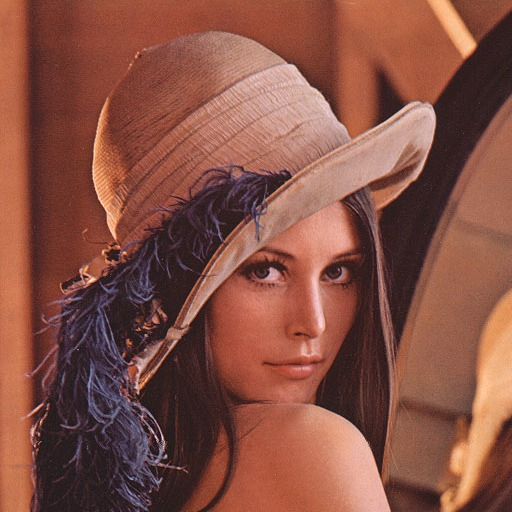
\includegraphics[width=15cm]{../../lena.jpg}
   \caption{Obraz poddawany obróbce}
\end{figure}


\newpage
\section{Sól i pieprz}
W losowych miejscach wartość wszystkich kanałów piksela ustalona zostaje na 0 lub maksymalną z zakresu.

\lstinputlisting[caption=Implementacja soli i pieprzu]{listingi/saltpepper.rb}

\begin{figure}[h!]
\begin{minipage}[t]{6cm}
\begin{center}
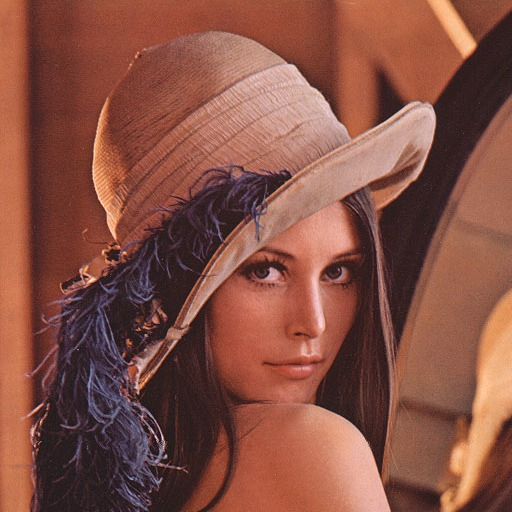
\includegraphics[width=6cm,clip]{../../lena.jpg}
\caption{orginal}
\end{center}
\end{minipage}
\hfill
\begin{minipage}[t]{6cm}
\begin{center}
\includegraphics[width=6cm,clip]{../out/saltpepper005.jpg}
\caption{freq 0.05}
\end{center}
\end{minipage}
\end{figure}

\begin{figure}[h!]
\begin{minipage}[t]{6cm}
\begin{center}
\includegraphics[width=6cm,clip]{../out/saltpepper01.jpg}
\caption{freq 0.1}
\end{center}
\end{minipage}
\hfill
\begin{minipage}[t]{6cm}
\begin{center}
\includegraphics[width=6cm,clip]{../out/saltpepper015.jpg}
\caption{freq 0.15}
\end{center}
\end{minipage}
\end{figure}


\section{Szum równomierny}
W losowych miejscach z zadaną częstotliwością freq należy zmienić wartości pikseli we wszystkich kanałach o z góry wybraną wartość z przedziału $ \langle -30, -21 \rangle \cup \langle 21, 30 \rangle $

\lstinputlisting[caption=Implementacja szumu rownomiernego]{listingi/regular_noise.rb}

\newpage
\begin{figure}[h!]
\begin{minipage}[t]{7.5cm}
\begin{center}
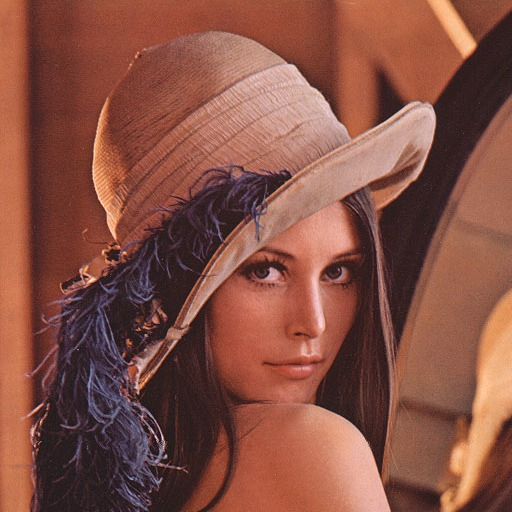
\includegraphics[width=7.5cm,clip]{../../lena.jpg}
\caption{orginal}
\end{center}
\end{minipage}
\hfill
\begin{minipage}[t]{7.5cm}
\begin{center}
\includegraphics[width=7.5cm,clip]{../out/regular_noise005.jpg}
\caption{freq 0.05, szum 6682}
\end{center}
\end{minipage}
\end{figure}

\begin{figure}[h!]
\begin{minipage}[t]{7.5cm}
\begin{center}
\includegraphics[width=7.5cm,clip]{../out/regular_noise015.jpg}
\caption{freq 0.15, szum 6425}
\end{center}
\end{minipage}
\hfill
\begin{minipage}[t]{7.5cm}
\begin{center}
\includegraphics[width=7.5cm,clip]{../out/regular_noise035.jpg}
\caption{freq 0.35, szum -5397}
\end{center}
\end{minipage}
\end{figure}


\newpage
\subsection{Szum równomierny w kanałach}
Operacja jest powtórzona, jednak tym razem poszczególne kanały zmieniają się o inną stałą wartość.

\begin{figure}[h!]
\begin{minipage}[t]{7.5cm}
\begin{center}
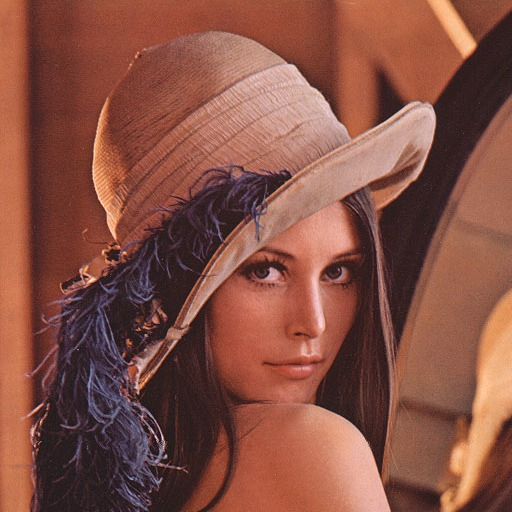
\includegraphics[width=7.5cm,clip]{../../lena.jpg}
\caption{orginal}
\end{center}
\end{minipage}
\hfill
\begin{minipage}[t]{7.5cm}
\begin{center}
\includegraphics[width=7.5cm,clip]{../out/regular_noise_ch005.jpg}
\caption{freq 0.05, szum r6168 g6682 b6168}
\end{center}
\end{minipage}
\end{figure}

\begin{figure}[h!]
\begin{minipage}[t]{7.5cm}
\begin{center}
\includegraphics[width=7.5cm,clip]{../out/regular_noise_ch015.jpg}
\caption{freq 0.15, szum r-6168 g-6425 b5911}
\end{center}
\end{minipage}
\hfill
\begin{minipage}[t]{7.5cm}
\begin{center}
\includegraphics[width=7.5cm,clip]{../out/regular_noise_ch035.jpg}
\caption{freq 0.35, szum r5654 g6682 b-5397}
\end{center}
\end{minipage}
\end{figure}

\newpage
\section{Odszumianie filtr medianowy}
Wartości każdego piksela zaszumionego obrazka wraz z jego otoczeniem szereguje się rosnąco w poszczególnych kanałach. Nową wartością piksela jest wartość środkowa w szeregu.

\lstinputlisting[caption=Utworzenie posortowanego szeregu z sasiedztwa]{listingi/median_filter_matrix.rb}
\lstinputlisting[caption=Implementacja filtru medianowego]{listingi/median_filter.rb}


\newpage
\subsection{Odszumianie soli i pieprzu o częstości 0.05}
\begin{figure}[h!]
\begin{minipage}[t]{7.5cm}
\begin{center}
\includegraphics[width=7.5cm,clip]{../out/saltpepper005.jpg}
\caption{obraz zaszumiony}
\end{center}
\end{minipage}
\hfill
\begin{minipage}[t]{7.5cm}
\begin{center}
\includegraphics[width=7.5cm,clip]{../out/saltpepper005__median_filter3.jpg}
\caption{filtr medianowy, 3x3}
\end{center}
\end{minipage}
\end{figure}

\begin{figure}[h!]
\begin{minipage}[t]{7.5cm}
\begin{center}
\includegraphics[width=7.5cm,clip]{../out/saltpepper005__median_filter5.jpg}
\caption{filtr medianowy, 5x5}
\end{center}
\end{minipage}
\hfill
\begin{minipage}[t]{7.5cm}
\begin{center}
\includegraphics[width=7.5cm,clip]{../out/saltpepper005__median_filter7.jpg}
\caption{filtr medianowy, 7x7}
\end{center}
\end{minipage}
\end{figure}


\newpage
\subsection{Odszumianie soli i pieprzu o częstości 0.1}
\begin{figure}[h!]
\begin{minipage}[t]{7.5cm}
\begin{center}
\includegraphics[width=7.5cm,clip]{../out/saltpepper01.jpg}
\caption{obraz zaszumiony}
\end{center}
\end{minipage}
\hfill
\begin{minipage}[t]{7.5cm}
\begin{center}
\includegraphics[width=7.5cm,clip]{../out/saltpepper01__median_filter3.jpg}
\caption{filtr medianowy, 3x3}
\end{center}
\end{minipage}
\end{figure}

\begin{figure}[h!]
\begin{minipage}[t]{7.5cm}
\begin{center}
\includegraphics[width=7.5cm,clip]{../out/saltpepper01__median_filter5.jpg}
\caption{filtr medianowy, 5x5}
\end{center}
\end{minipage}
\hfill
\begin{minipage}[t]{7.5cm}
\begin{center}
\includegraphics[width=7.5cm,clip]{../out/saltpepper01__median_filter7.jpg}
\caption{filtr medianowy, 7x7}
\end{center}
\end{minipage}
\end{figure}


\newpage
\subsection{Odszumianie soli i pieprzu o częstości 0.15}
\begin{figure}[h!]
\begin{minipage}[t]{7.5cm}
\begin{center}
\includegraphics[width=7.5cm,clip]{../out/saltpepper015.jpg}
\caption{obraz zaszumiony}
\end{center}
\end{minipage}
\hfill
\begin{minipage}[t]{7.5cm}
\begin{center}
\includegraphics[width=7.5cm,clip]{../out/saltpepper015__median_filter3.jpg}
\caption{filtr medianowy, 3x3}
\end{center}
\end{minipage}
\end{figure}

\begin{figure}[h!]
\begin{minipage}[t]{7.5cm}
\begin{center}
\includegraphics[width=7.5cm,clip]{../out/saltpepper015__median_filter5.jpg}
\caption{filtr medianowy, 5x5}
\end{center}
\end{minipage}
\hfill
\begin{minipage}[t]{7.5cm}
\begin{center}
\includegraphics[width=7.5cm,clip]{../out/saltpepper015__median_filter7.jpg}
\caption{filtr medianowy, 7x7}
\end{center}
\end{minipage}
\end{figure}


\newpage
\subsection{Odszumianie szumu równomiernego jednokanałowego o częstości 0.1}
\begin{figure}[h!]
\begin{minipage}[t]{7.5cm}
\begin{center}
\includegraphics[width=7.5cm,clip]{../out/regular_noise_ch01.jpg}
\caption{obraz zaszumiony}
\end{center}
\end{minipage}
\hfill
\begin{minipage}[t]{7.5cm}
\begin{center}
\includegraphics[width=7.5cm,clip]{../out/regular_noise01__median_filter3.jpg}
\caption{filtr medianowy, 3x3}
\end{center}
\end{minipage}
\end{figure}

\begin{figure}[h!]
\begin{minipage}[t]{7.5cm}
\begin{center}
\includegraphics[width=7.5cm,clip]{../out/regular_noise01__median_filter5.jpg}
\caption{filtr medianowy, 5x5}
\end{center}
\end{minipage}
\hfill
\begin{minipage}[t]{7.5cm}
\begin{center}
\includegraphics[width=7.5cm,clip]{../out/regular_noise01__median_filter7.jpg}
\caption{filtr medianowy, 7x7}
\end{center}
\end{minipage}
\end{figure}


\newpage
\subsection{Odszumianie szumu równomiernego jednokanałowego o częstości 0.35}
\begin{figure}[h!]
\begin{minipage}[t]{7.5cm}
\begin{center}
\includegraphics[width=7.5cm,clip]{../out/regular_noise_ch035.jpg}
\caption{obraz zaszumiony}
\end{center}
\end{minipage}
\hfill
\begin{minipage}[t]{7.5cm}
\begin{center}
\includegraphics[width=7.5cm,clip]{../out/regular_noise035__median_filter3.jpg}
\caption{filtr medianowy, 3x3}
\end{center}
\end{minipage}
\end{figure}

\begin{figure}[h!]
\begin{minipage}[t]{7.5cm}
\begin{center}
\includegraphics[width=7.5cm,clip]{../out/regular_noise035__median_filter5.jpg}
\caption{filtr medianowy, 5x5}
\end{center}
\end{minipage}
\hfill
\begin{minipage}[t]{7.5cm}
\begin{center}
\includegraphics[width=7.5cm,clip]{../out/regular_noise035__median_filter7.jpg}
\caption{filtr medianowy, 7x7}
\end{center}
\end{minipage}
\end{figure}


\newpage
\subsection{Odszumianie szumu równomiernego różnokanałowego o częstości 0.1}
\begin{figure}[h!]
\begin{minipage}[t]{7.5cm}
\begin{center}
\includegraphics[width=7.5cm,clip]{../out/regular_noise_ch01.jpg}
\caption{obraz zaszumiony}
\end{center}
\end{minipage}
\hfill
\begin{minipage}[t]{7.5cm}
\begin{center}
\includegraphics[width=7.5cm,clip]{../out/regular_noise_ch01__median_filter3.jpg}
\caption{filtr medianowy, 3x3}
\end{center}
\end{minipage}
\end{figure}

\begin{figure}[h!]
\begin{minipage}[t]{7.5cm}
\begin{center}
\includegraphics[width=7.5cm,clip]{../out/regular_noise_ch01__median_filter5.jpg}
\caption{filtr medianowy, 5x5}
\end{center}
\end{minipage}
\hfill
\begin{minipage}[t]{7.5cm}
\begin{center}
\includegraphics[width=7.5cm,clip]{../out/regular_noise_ch01__median_filter7.jpg}
\caption{filtr medianowy, 7x7}
\end{center}
\end{minipage}
\end{figure}


\newpage
\subsection{Odszumianie szumu równomiernego różnokanałowego o częstości 0.35}
\begin{figure}[h!]
\begin{minipage}[t]{7.5cm}
\begin{center}
\includegraphics[width=7.5cm,clip]{../out/regular_noise_ch035.jpg}
\caption{obraz zaszumiony}
\end{center}
\end{minipage}
\hfill
\begin{minipage}[t]{7.5cm}
\begin{center}
\includegraphics[width=7.5cm,clip]{../out/regular_noise_ch035__median_filter3.jpg}
\caption{filtr medianowy, 3x3}
\end{center}
\end{minipage}
\end{figure}

\begin{figure}[h!]
\begin{minipage}[t]{7.5cm}
\begin{center}
\includegraphics[width=7.5cm,clip]{../out/regular_noise_ch035__median_filter5.jpg}
\caption{filtr medianowy, 5x5}
\end{center}
\end{minipage}
\hfill
\begin{minipage}[t]{7.5cm}
\begin{center}
\includegraphics[width=7.5cm,clip]{../out/regular_noise_ch035__median_filter7.jpg}
\caption{filtr medianowy, 7x7}
\end{center}
\end{minipage}
\end{figure}









\newpage
\section{Odszumianie filtr medianowy warunkowy}
Tym razem sprawdzane jest czy pierwotna wartość piksela zawiera się w dwóch skrajnych końcach szeregu. Jeśli tak - stara wartość jest pozostawiana. Inaczej postępowanie pozostaje jak poprzednio i wybierany jest środkowa wartość z szeregu. Działanie pozwala uniknąć wyrównywania pikseli znacznie różniących się od otoczenia.

\lstinputlisting[caption=Implementacja filtru medianowego warunkowego]{listingi/median_filter_limited.rb}


\newpage
\subsection{Odszumianie soli i pieprzu o częstości 0.05}
\begin{figure}[h!]
\begin{minipage}[t]{7.5cm}
\begin{center}
\includegraphics[width=7.5cm,clip]{../out/saltpepper005.jpg}
\caption{obraz zaszumiony}
\end{center}
\end{minipage}
\hfill
\begin{minipage}[t]{7.5cm}
\begin{center}
\includegraphics[width=7.5cm,clip]{../out/saltpepper005__median_filter_limited3.jpg}
\caption{filtr medianowy warunkowy, 3x3}
\end{center}
\end{minipage}
\end{figure}

\begin{figure}[h!]
\begin{minipage}[t]{7.5cm}
\begin{center}
\includegraphics[width=7.5cm,clip]{../out/saltpepper005__median_filter_limited5.jpg}
\caption{filtr medianowy warunkowy, 5x5}
\end{center}
\end{minipage}
\hfill
\begin{minipage}[t]{7.5cm}
\begin{center}
\includegraphics[width=7.5cm,clip]{../out/saltpepper005__median_filter_limited7.jpg}
\caption{filtr medianowy warunkowy, 7x7}
\end{center}
\end{minipage}
\end{figure}


\newpage
\subsection{Odszumianie soli i pieprzu o częstości 0.1}
\begin{figure}[h!]
\begin{minipage}[t]{7.5cm}
\begin{center}
\includegraphics[width=7.5cm,clip]{../out/saltpepper01.jpg}
\caption{obraz zaszumiony}
\end{center}
\end{minipage}
\hfill
\begin{minipage}[t]{7.5cm}
\begin{center}
\includegraphics[width=7.5cm,clip]{../out/saltpepper01__median_filter_limited3.jpg}
\caption{filtr medianowy warunkowy, 3x3}
\end{center}
\end{minipage}
\end{figure}

\begin{figure}[h!]
\begin{minipage}[t]{7.5cm}
\begin{center}
\includegraphics[width=7.5cm,clip]{../out/saltpepper01__median_filter_limited5.jpg}
\caption{filtr medianowy warunkowy, 5x5}
\end{center}
\end{minipage}
\hfill
\begin{minipage}[t]{7.5cm}
\begin{center}
\includegraphics[width=7.5cm,clip]{../out/saltpepper01__median_filter_limited7.jpg}
\caption{filtr medianowy warunkowy, 7x7}
\end{center}
\end{minipage}
\end{figure}


\newpage
\subsection{Odszumianie soli i pieprzu o częstości 0.15}
\begin{figure}[h!]
\begin{minipage}[t]{7.5cm}
\begin{center}
\includegraphics[width=7.5cm,clip]{../out/saltpepper015.jpg}
\caption{obraz zaszumiony}
\end{center}
\end{minipage}
\hfill
\begin{minipage}[t]{7.5cm}
\begin{center}
\includegraphics[width=7.5cm,clip]{../out/saltpepper015__median_filter_limited3.jpg}
\caption{filtr medianowy warunkowy, 3x3}
\end{center}
\end{minipage}
\end{figure}

\begin{figure}[h!]
\begin{minipage}[t]{7.5cm}
\begin{center}
\includegraphics[width=7.5cm,clip]{../out/saltpepper015__median_filter_limited5.jpg}
\caption{filtr medianowy warunkowy, 5x5}
\end{center}
\end{minipage}
\hfill
\begin{minipage}[t]{7.5cm}
\begin{center}
\includegraphics[width=7.5cm,clip]{../out/saltpepper015__median_filter_limited7.jpg}
\caption{filtr medianowy warunkowy, 7x7}
\end{center}
\end{minipage}
\end{figure}


\newpage
\subsection{Odszumianie szumu równomiernego jednokanałowego o częstości 0.1}
\begin{figure}[h!]
\begin{minipage}[t]{7.5cm}
\begin{center}
\includegraphics[width=7.5cm,clip]{../out/regular_noise_ch01.jpg}
\caption{obraz zaszumiony}
\end{center}
\end{minipage}
\hfill
\begin{minipage}[t]{7.5cm}
\begin{center}
\includegraphics[width=7.5cm,clip]{../out/regular_noise01__median_filter_limited3.jpg}
\caption{filtr medianowy warunkowy, 3x3}
\end{center}
\end{minipage}
\end{figure}

\begin{figure}[h!]
\begin{minipage}[t]{7.5cm}
\begin{center}
\includegraphics[width=7.5cm,clip]{../out/regular_noise01__median_filter_limited5.jpg}
\caption{filtr medianowy warunkowy, 5x5}
\end{center}
\end{minipage}
\hfill
\begin{minipage}[t]{7.5cm}
\begin{center}
\includegraphics[width=7.5cm,clip]{../out/regular_noise01__median_filter_limited7.jpg}
\caption{filtr medianowy warunkowy, 7x7}
\end{center}
\end{minipage}
\end{figure}


\newpage
\subsection{Odszumianie szumu równomiernego jednokanałowego o częstości 0.35}
\begin{figure}[h!]
\begin{minipage}[t]{7.5cm}
\begin{center}
\includegraphics[width=7.5cm,clip]{../out/regular_noise_ch035.jpg}
\caption{obraz zaszumiony}
\end{center}
\end{minipage}
\hfill
\begin{minipage}[t]{7.5cm}
\begin{center}
\includegraphics[width=7.5cm,clip]{../out/regular_noise035__median_filter_limited3.jpg}
\caption{filtr medianowy warunkowy, 3x3}
\end{center}
\end{minipage}
\end{figure}

\begin{figure}[h!]
\begin{minipage}[t]{7.5cm}
\begin{center}
\includegraphics[width=7.5cm,clip]{../out/regular_noise035__median_filter_limited5.jpg}
\caption{filtr medianowy warunkowy, 5x5}
\end{center}
\end{minipage}
\hfill
\begin{minipage}[t]{7.5cm}
\begin{center}
\includegraphics[width=7.5cm,clip]{../out/regular_noise035__median_filter_limited7.jpg}
\caption{filtr medianowy warunkowy, 7x7}
\end{center}
\end{minipage}
\end{figure}


\newpage
\subsection{Odszumianie szumu równomiernego różnokanałowego o częstości 0.1}
\begin{figure}[h!]
\begin{minipage}[t]{7.5cm}
\begin{center}
\includegraphics[width=7.5cm,clip]{../out/regular_noise_ch01.jpg}
\caption{obraz zaszumiony}
\end{center}
\end{minipage}
\hfill
\begin{minipage}[t]{7.5cm}
\begin{center}
\includegraphics[width=7.5cm,clip]{../out/regular_noise_ch01__median_filter_limited3.jpg}
\caption{filtr medianowy warunkowy, 3x3}
\end{center}
\end{minipage}
\end{figure}

\begin{figure}[h!]
\begin{minipage}[t]{7.5cm}
\begin{center}
\includegraphics[width=7.5cm,clip]{../out/regular_noise_ch01__median_filter_limited5.jpg}
\caption{filtr medianowy warunkowy, 5x5}
\end{center}
\end{minipage}
\hfill
\begin{minipage}[t]{7.5cm}
\begin{center}
\includegraphics[width=7.5cm,clip]{../out/regular_noise_ch01__median_filter_limited7.jpg}
\caption{filtr medianowy warunkowy, 7x7}
\end{center}
\end{minipage}
\end{figure}


\newpage
\subsection{Odszumianie szumu równomiernego różnokanałowego o częstości 0.35}
\begin{figure}[h!]
\begin{minipage}[t]{7.5cm}
\begin{center}
\includegraphics[width=7.5cm,clip]{../out/regular_noise_ch035.jpg}
\caption{obraz zaszumiony}
\end{center}
\end{minipage}
\hfill
\begin{minipage}[t]{7.5cm}
\begin{center}
\includegraphics[width=7.5cm,clip]{../out/regular_noise_ch035__median_filter_limited3.jpg}
\caption{filtr medianowy warunkowy, 3x3}
\end{center}
\end{minipage}
\end{figure}

\begin{figure}[h!]
\begin{minipage}[t]{7.5cm}
\begin{center}
\includegraphics[width=7.5cm,clip]{../out/regular_noise_ch035__median_filter_limited5.jpg}
\caption{filtr medianowy warunkowy, 5x5}
\end{center}
\end{minipage}
\hfill
\begin{minipage}[t]{7.5cm}
\begin{center}
\includegraphics[width=7.5cm,clip]{../out/regular_noise_ch035__median_filter_limited7.jpg}
\caption{filtr medianowy warunkowy, 7x7}
\end{center}
\end{minipage}
\end{figure}









\newpage
\section{Odszumianie filtr uśredniający}
Wartości każdego piksela zaszumionego obrazka wraz z jego otoczeniem poddaje się uśrednieniu.

\lstinputlisting[caption=Implementacja filtru usredniajacego]{listingi/average_filter.rb}


\newpage
\subsection{Odszumianie soli i pieprzu o częstości 0.05}
\begin{figure}[h!]
\begin{minipage}[t]{7.5cm}
\begin{center}
\includegraphics[width=7.5cm,clip]{../out/saltpepper005.jpg}
\caption{obraz zaszumiony}
\end{center}
\end{minipage}
\hfill
\begin{minipage}[t]{7.5cm}
\begin{center}
\includegraphics[width=7.5cm,clip]{../out/saltpepper005__average_filter3.jpg}
\caption{filtr usredniajacy, 3x3}
\end{center}
\end{minipage}
\end{figure}

\begin{figure}[h!]
\begin{minipage}[t]{7.5cm}
\begin{center}
\includegraphics[width=7.5cm,clip]{../out/saltpepper005__average_filter5.jpg}
\caption{filtr usredniajacy, 5x5}
\end{center}
\end{minipage}
\hfill
\begin{minipage}[t]{7.5cm}
\begin{center}
\includegraphics[width=7.5cm,clip]{../out/saltpepper005__average_filter7.jpg}
\caption{filtr usredniajacy, 7x7}
\end{center}
\end{minipage}
\end{figure}


\newpage
\subsection{Odszumianie soli i pieprzu o częstości 0.1}
\begin{figure}[h!]
\begin{minipage}[t]{7.5cm}
\begin{center}
\includegraphics[width=7.5cm,clip]{../out/saltpepper01.jpg}
\caption{obraz zaszumiony}
\end{center}
\end{minipage}
\hfill
\begin{minipage}[t]{7.5cm}
\begin{center}
\includegraphics[width=7.5cm,clip]{../out/saltpepper01__average_filter3.jpg}
\caption{filtr usredniajacy, 3x3}
\end{center}
\end{minipage}
\end{figure}

\begin{figure}[h!]
\begin{minipage}[t]{7.5cm}
\begin{center}
\includegraphics[width=7.5cm,clip]{../out/saltpepper01__average_filter5.jpg}
\caption{filtr usredniajacy, 5x5}
\end{center}
\end{minipage}
\hfill
\begin{minipage}[t]{7.5cm}
\begin{center}
\includegraphics[width=7.5cm,clip]{../out/saltpepper01__average_filter7.jpg}
\caption{filtr usredniajacy, 7x7}
\end{center}
\end{minipage}
\end{figure}


\newpage
\subsection{Odszumianie soli i pieprzu o częstości 0.15}
\begin{figure}[h!]
\begin{minipage}[t]{7.5cm}
\begin{center}
\includegraphics[width=7.5cm,clip]{../out/saltpepper015.jpg}
\caption{obraz zaszumiony}
\end{center}
\end{minipage}
\hfill
\begin{minipage}[t]{7.5cm}
\begin{center}
\includegraphics[width=7.5cm,clip]{../out/saltpepper015__average_filter3.jpg}
\caption{filtr usredniajacy, 3x3}
\end{center}
\end{minipage}
\end{figure}

\begin{figure}[h!]
\begin{minipage}[t]{7.5cm}
\begin{center}
\includegraphics[width=7.5cm,clip]{../out/saltpepper015__average_filter5.jpg}
\caption{filtr usredniajacy, 5x5}
\end{center}
\end{minipage}
\hfill
\begin{minipage}[t]{7.5cm}
\begin{center}
\includegraphics[width=7.5cm,clip]{../out/saltpepper015__average_filter7.jpg}
\caption{filtr usredniajacy, 7x7}
\end{center}
\end{minipage}
\end{figure}


\newpage
\subsection{Odszumianie szumu równomiernego jednokanałowego o częstości 0.1}
\begin{figure}[h!]
\begin{minipage}[t]{7.5cm}
\begin{center}
\includegraphics[width=7.5cm,clip]{../out/regular_noise_ch01.jpg}
\caption{obraz zaszumiony}
\end{center}
\end{minipage}
\hfill
\begin{minipage}[t]{7.5cm}
\begin{center}
\includegraphics[width=7.5cm,clip]{../out/regular_noise01__average_filter3.jpg}
\caption{filtr usredniajacy, 3x3}
\end{center}
\end{minipage}
\end{figure}

\begin{figure}[h!]
\begin{minipage}[t]{7.5cm}
\begin{center}
\includegraphics[width=7.5cm,clip]{../out/regular_noise01__average_filter5.jpg}
\caption{filtr usredniajacy, 5x5}
\end{center}
\end{minipage}
\hfill
\begin{minipage}[t]{7.5cm}
\begin{center}
\includegraphics[width=7.5cm,clip]{../out/regular_noise01__average_filter7.jpg}
\caption{filtr usredniajacy, 7x7}
\end{center}
\end{minipage}
\end{figure}


\newpage
\subsection{Odszumianie szumu równomiernego jednokanałowego o częstości 0.35}
\begin{figure}[h!]
\begin{minipage}[t]{7.5cm}
\begin{center}
\includegraphics[width=7.5cm,clip]{../out/regular_noise_ch035.jpg}
\caption{obraz zaszumiony}
\end{center}
\end{minipage}
\hfill
\begin{minipage}[t]{7.5cm}
\begin{center}
\includegraphics[width=7.5cm,clip]{../out/regular_noise035__average_filter3.jpg}
\caption{filtr usredniajacy, 3x3}
\end{center}
\end{minipage}
\end{figure}

\begin{figure}[h!]
\begin{minipage}[t]{7.5cm}
\begin{center}
\includegraphics[width=7.5cm,clip]{../out/regular_noise035__average_filter5.jpg}
\caption{filtr usredniajacy, 5x5}
\end{center}
\end{minipage}
\hfill
\begin{minipage}[t]{7.5cm}
\begin{center}
\includegraphics[width=7.5cm,clip]{../out/regular_noise035__average_filter7.jpg}
\caption{filtr usredniajacy, 7x7}
\end{center}
\end{minipage}
\end{figure}


\newpage
\subsection{Odszumianie szumu równomiernego różnokanałowego o częstości 0.1}
\begin{figure}[h!]
\begin{minipage}[t]{7.5cm}
\begin{center}
\includegraphics[width=7.5cm,clip]{../out/regular_noise_ch01.jpg}
\caption{obraz zaszumiony}
\end{center}
\end{minipage}
\hfill
\begin{minipage}[t]{7.5cm}
\begin{center}
\includegraphics[width=7.5cm,clip]{../out/regular_noise_ch01__average_filter3.jpg}
\caption{filtr usredniajacy, 3x3}
\end{center}
\end{minipage}
\end{figure}

\begin{figure}[h!]
\begin{minipage}[t]{7.5cm}
\begin{center}
\includegraphics[width=7.5cm,clip]{../out/regular_noise_ch01__average_filter5.jpg}
\caption{filtr usredniajacy, 5x5}
\end{center}
\end{minipage}
\hfill
\begin{minipage}[t]{7.5cm}
\begin{center}
\includegraphics[width=7.5cm,clip]{../out/regular_noise_ch01__average_filter7.jpg}
\caption{filtr usredniajacy, 7x7}
\end{center}
\end{minipage}
\end{figure}


\newpage
\subsection{Odszumianie szumu równomiernego różnokanałowego o częstości 0.35}
\begin{figure}[h!]
\begin{minipage}[t]{7.5cm}
\begin{center}
\includegraphics[width=7.5cm,clip]{../out/regular_noise_ch035.jpg}
\caption{obraz zaszumiony}
\end{center}
\end{minipage}
\hfill
\begin{minipage}[t]{7.5cm}
\begin{center}
\includegraphics[width=7.5cm,clip]{../out/regular_noise_ch035__average_filter3.jpg}
\caption{filtr usredniajacy, 3x3}
\end{center}
\end{minipage}
\end{figure}

\begin{figure}[h!]
\begin{minipage}[t]{7.5cm}
\begin{center}
\includegraphics[width=7.5cm,clip]{../out/regular_noise_ch035__average_filter5.jpg}
\caption{filtr usredniajacy, 5x5}
\end{center}
\end{minipage}
\hfill
\begin{minipage}[t]{7.5cm}
\begin{center}
\includegraphics[width=7.5cm,clip]{../out/regular_noise_ch035__average_filter7.jpg}
\caption{filtr usredniajacy, 7x7}
\end{center}
\end{minipage}
\end{figure}



\section{Wnioski}
Widać, że nie ma jednej optymalnej metody do odszumienia każdego rodzaju nieczystości. Dobór metody zależy od rodzaju szumu. Zamieszczam efekty działania filtrów o najlepszych rezultatach.


\newpage
\subsection{Odszumianie soli i pieprzu o częstości 0.05}
\begin{figure}[h!]
\begin{minipage}[t]{7.5cm}
\begin{center}
\includegraphics[width=7.5cm,clip]{../out/saltpepper005.jpg}
\caption{obraz zaszumiony}
\end{center}
\end{minipage}
\hfill
\begin{minipage}[t]{7.5cm}
\begin{center}
\includegraphics[width=7.5cm,clip]{../out/saltpepper005__median_filter3.jpg}
\caption{filtr medianowy, 3x3}
\end{center}
\end{minipage}
\end{figure}

\begin{figure}[h!]
\begin{minipage}[t]{7.5cm}
\begin{center}
\includegraphics[width=7.5cm,clip]{../out/saltpepper005__median_filter_limited5.jpg}
\caption{filtr medianowy warunkowy, 5x5}
\end{center}
\end{minipage}
\hfill
\begin{minipage}[t]{7.5cm}
\begin{center}
\includegraphics[width=7.5cm,clip]{../out/saltpepper005__average_filter7.jpg}
\caption{filtr usredniajacy, 7x7}
\end{center}
\end{minipage}
\end{figure}


\newpage
\subsection{Odszumianie soli i pieprzu o częstości 0.1}
\begin{figure}[h!]
\begin{minipage}[t]{7.5cm}
\begin{center}
\includegraphics[width=7.5cm,clip]{../out/saltpepper01.jpg}
\caption{obraz zaszumiony}
\end{center}
\end{minipage}
\hfill
\begin{minipage}[t]{7.5cm}
\begin{center}
\includegraphics[width=7.5cm,clip]{../out/saltpepper01__median_filter3.jpg}
\caption{filtr medianowy, 3x3}
\end{center}
\end{minipage}
\end{figure}

\begin{figure}[h!]
\begin{minipage}[t]{7.5cm}
\begin{center}
\includegraphics[width=7.5cm,clip]{../out/saltpepper01__median_filter_limited5.jpg}
\caption{filtr medianowy warunkowy, 5x5}
\end{center}
\end{minipage}
\hfill
\begin{minipage}[t]{7.5cm}
\begin{center}
\includegraphics[width=7.5cm,clip]{../out/saltpepper01__average_filter7.jpg}
\caption{filtr usredniajacy, 7x7}
\end{center}
\end{minipage}
\end{figure}


\newpage
\subsection{Odszumianie soli i pieprzu o częstości 0.15}
\begin{figure}[h!]
\begin{minipage}[t]{7.5cm}
\begin{center}
\includegraphics[width=7.5cm,clip]{../out/saltpepper015.jpg}
\caption{obraz zaszumiony}
\end{center}
\end{minipage}
\hfill
\begin{minipage}[t]{7.5cm}
\begin{center}
\includegraphics[width=7.5cm,clip]{../out/saltpepper015__median_filter3.jpg}
\caption{filtr medianowy, 3x3}
\end{center}
\end{minipage}
\end{figure}

\begin{figure}[h!]
\begin{minipage}[t]{7.5cm}
\begin{center}
\includegraphics[width=7.5cm,clip]{../out/saltpepper015__median_filter_limited7.jpg}
\caption{filtr medianowy warunkowy, 7x7}
\end{center}
\end{minipage}
\hfill
\begin{minipage}[t]{7.5cm}
\begin{center}
\includegraphics[width=7.5cm,clip]{../out/saltpepper015__average_filter7.jpg}
\caption{filtr usredniajacy, 7x7}
\end{center}
\end{minipage}
\end{figure}


Z solą i pieprzem najlepiej radzi sobie prosty filtr medianowy. Filtr medianowy warunkowy pozostawia starą wartość kanału piksela jeśli zbytnio się ona różni od swojego sąsiedztwa. A szum typu sól i pieprz wprowadza właśnie piksele skrajnie się różniące. Pomaga powiększenie siatki do rozmiarów 5x5. Filtr uśredniający zupełnie się nie sprawdza. W tym przypadku szum nabardziej wtapiający się w tło pokazuje siatka 7x7, jednakże obraz staje się niewyraźny. Tak duża siatka w przypadku filtru medianowego niewarunkowego powoduje rozmycie do stopnia przypominającego obraz malowany farbami olejnymi. Warunkowość ogranicza ten efekt uboczny.




\newpage
\subsection{Odszumianie zanieczyszczeń równomiernych jednokanałowych o częstości 0.1}
\begin{figure}[h!]
\begin{minipage}[t]{7.5cm}
\begin{center}
\includegraphics[width=7.5cm,clip]{../out/regular_noise01.jpg}
\caption{obraz zaszumiony}
\end{center}
\end{minipage}
\hfill
\begin{minipage}[t]{7.5cm}
\begin{center}
\includegraphics[width=7.5cm,clip]{../out/regular_noise01__median_filter3.jpg}
\caption{filtr medianowy, 3x3}
\end{center}
\end{minipage}
\end{figure}

\begin{figure}[h!]
\begin{minipage}[t]{7.5cm}
\begin{center}
\includegraphics[width=7.5cm,clip]{../out/regular_noise01__median_filter_limited3.jpg}
\caption{filtr medianowy warunkowy, 3x3}
\end{center}
\end{minipage}
\hfill
\begin{minipage}[t]{7.5cm}
\begin{center}
\includegraphics[width=7.5cm,clip]{../out/regular_noise01__average_filter3.jpg}
\caption{filtr usredniajacy, 3x3}
\end{center}
\end{minipage}
\end{figure}


\newpage
\subsection{Odszumianie zanieczyszczeń równomiernych jednokanałowych o częstości 0.35}
\begin{figure}[h!]
\begin{minipage}[t]{7.5cm}
\begin{center}
\includegraphics[width=7.5cm,clip]{../out/regular_noise035.jpg}
\caption{obraz zaszumiony}
\end{center}
\end{minipage}
\hfill
\begin{minipage}[t]{7.5cm}
\begin{center}
\includegraphics[width=7.5cm,clip]{../out/regular_noise035__median_filter3.jpg}
\caption{filtr medianowy, 3x3}
\end{center}
\end{minipage}
\end{figure}

\begin{figure}[h!]
\begin{minipage}[t]{7.5cm}
\begin{center}
\includegraphics[width=7.5cm,clip]{../out/regular_noise035__median_filter_limited5.jpg}
\caption{filtr medianowy warunkowy, 5x5}
\end{center}
\end{minipage}
\hfill
\begin{minipage}[t]{7.5cm}
\begin{center}
\includegraphics[width=7.5cm,clip]{../out/regular_noise035__average_filter5.jpg}
\caption{filtr usredniajacy, 5x5}
\end{center}
\end{minipage}
\end{figure}


\newpage
\subsection{Odszumianie zanieczyszczeń równomiernych różnokanałowych o częstości 0.1}
\begin{figure}[h!]
\begin{minipage}[t]{7.5cm}
\begin{center}
\includegraphics[width=7.5cm,clip]{../out/regular_noise_ch01.jpg}
\caption{obraz zaszumiony}
\end{center}
\end{minipage}
\hfill
\begin{minipage}[t]{7.5cm}
\begin{center}
\includegraphics[width=7.5cm,clip]{../out/regular_noise_ch01__median_filter3.jpg}
\caption{filtr medianowy, 3x3}
\end{center}
\end{minipage}
\end{figure}

\begin{figure}[h!]
\begin{minipage}[t]{7.5cm}
\begin{center}
\includegraphics[width=7.5cm,clip]{../out/regular_noise_ch01__median_filter_limited3.jpg}
\caption{filtr medianowy warunkowy, 3x3}
\end{center}
\end{minipage}
\hfill
\begin{minipage}[t]{7.5cm}
\begin{center}
\includegraphics[width=7.5cm,clip]{../out/regular_noise_ch01__average_filter3.jpg}
\caption{filtr usredniajacy, 3x3}
\end{center}
\end{minipage}
\end{figure}


\newpage
\subsection{Odszumianie zanieczyszczeń równomiernych różnokanałowych o częstości 0.35}
\begin{figure}[h!]
\begin{minipage}[t]{7.5cm}
\begin{center}
\includegraphics[width=7.5cm,clip]{../out/regular_noise_ch035.jpg}
\caption{obraz zaszumiony}
\end{center}
\end{minipage}
\hfill
\begin{minipage}[t]{7.5cm}
\begin{center}
\includegraphics[width=7.5cm,clip]{../out/regular_noise_ch035__median_filter5.jpg}
\caption{filtr medianowy, 5x5}
\end{center}
\end{minipage}
\end{figure}

\begin{figure}[h!]
\begin{minipage}[t]{7.5cm}
\begin{center}
\includegraphics[width=7.5cm,clip]{../out/regular_noise_ch035__median_filter_limited7.jpg}
\caption{filtr medianowy warunkowy, 7x7}
\end{center}
\end{minipage}
\hfill
\begin{minipage}[t]{7.5cm}
\begin{center}
\includegraphics[width=7.5cm,clip]{../out/regular_noise_ch035__average_filter7.jpg}
\caption{filtr usredniajacy, 7x7}
\end{center}
\end{minipage}
\end{figure}

Szum rownomierny zarówno jednokanałowy jak i różnokanałowy o częstotliwości 10\% jest niezauważalny, dlatego do odszumienia go wystarczą najmniejsze siatki filtrów. Szum na poziomie 35\% uwidacznia się. Jeśli jest jednokanałowy niwelują go skutecznie siatki 3x3 - 5x5, różnokanałowy wymaga większych siatek 5x5 - 7x7. Filtr medianowy niewarunkowy potrzebuje najmniejszych siatek, jednak uzyskuje podobne rezultaty co filtr medianowy warunkowy o większej siatce. Filtr uśredniający ponownie daje najgorsze rezultaty. 

\end{document}
